\tikzsetnextfilename{mr_transverse_magnetization_recovery_2tissues}
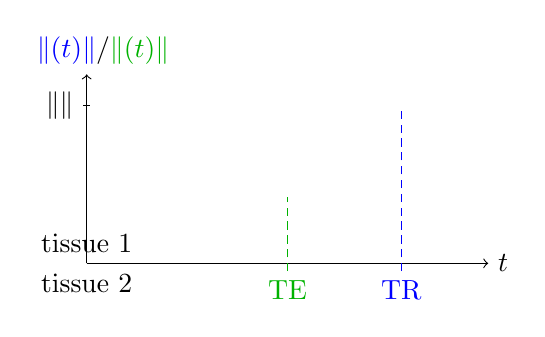
\begin{tikzpicture}[yscale=2,xscale=0.85]
	\draw[->] (0, 0) -- (0, 1.2) node [above right,xshift=-5ex] {{\color{blue}$\Vert\magnlong(t)\Vert$}/{\color{green!70!black}$\Vert\magntrans(t)\Vert$}};
	\draw[->] (0, 0) -- (6, 0) node [right] {$t$};
	% \draw[densely dashed] (1, -0.05) node [below] {$\transtime = 45\,\textrm{ms}$} -- (1, 0.37);
	% \draw[densely dashed] (5, -0.05) node [below] {$5\transtime = 225\,\textrm{ms}$} -- (5, 0.03);
	\draw[domain=0:5.5,samples=100,very thick, green!70!black] plot[id=mr_t2_recovery_tissue1] function{exp(-x/1.5)};
	\draw[domain=0:5.5,samples=100,very thick, green!70!black,densely dotted] plot[id=mr_t2_recovery_tissue2] function{exp(-x/3.5)};
	\draw[domain=0:5.5,samples=100,very thick, blue] plot[id=mr_t1_recovery_tissue1] function{1-exp(-x/0.45)} node [above, black] {tissue 1};
	\draw[domain=0:5.5,samples=100,very thick, blue, densely dotted] plot[id=mr_t1_recovery_tissue2] function{1-exp(-x/2)} node [below, black] {tissue 2};
	\draw[densely dashed] (-0.05, 1) node [left] {$\Vert\magnzero{}\Vert$} -- (0.05, 1);
	\draw[densely dashed,green!70!black] (3, -0.05) node [below] {TE} -- (3, 0.424);
	\draw[densely dashed,blue] (4.7, -0.05) node [below] {TR} -- (4.7, 1);
\end{tikzpicture}